\documentclass[12pt]{zettel}

\usepackage{pdfpages}
\usepackage{booktabs}

\usepackage{geometry}
\geometry{tmargin=2cm,bmargin=2cm,lmargin=3cm,rmargin=3cm}

\renewcommand{\gregor}{\put(13.2,-3.0){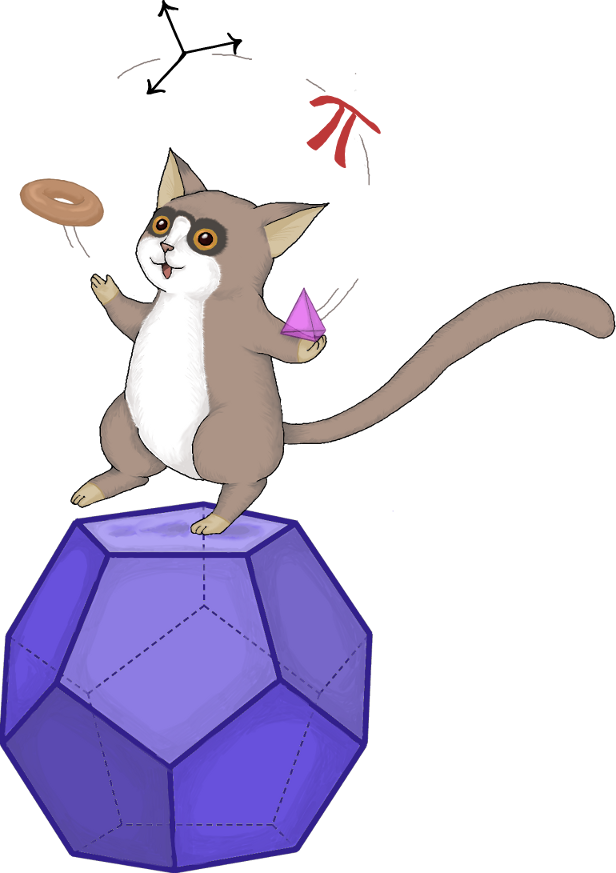
\includegraphics[scale=0.18]{cover}}}

\usepackage{framed}
\definecolor{shadecolor}{rgb}{.97,.97,.97}

\begin{document}

\renewcommand{\betreff}{}

\makeletterhead{}

\vspace{-2em}

\begin{center}
  \Large\textbf{\textsf{Bewerbung um den Witty-Jugendförderpreis 2014: \\
  Matheschülerzirkel Augsburg }}
\end{center}

Aus der Anforderungsbeschreibung: "`Das Projekt soll
Kindern/Jugendlichen Selbstwertgefühl vermitteln, sie fördern und nachhaltig
Hilfe zur Selbsthilfe bieten."'

\begin{itemize}
\item Information über Verein und Aktivitäten inkl. evtl. Presseberichte
\item Wie setzen sich die rd. 50 TeilnehmerInnen am Mathematikcamp zusammen? Kann
man sich einfach bewerben - läuft es über Lehrer bzw. Schulen?
\item Wie sieht es mit der "`Nachhaltigkeit"' aus? d.h. wie geht es weiter, wenn
einzelne Schüler richtig +Feuer fangen und Begabung zeigen?
\item Wie lauten Ihre Ziele bei diesen Aktivitäten und Projekten? Gibt es zu
wenig Mathematikstudenten und setzen Sie deshalb bereits so früh an?
\item Das Preisgeld beträgt 10.000 Euro. Für das Camp benötigen Sie 7000,--. Wie
würden Sie das restliche Preisgeld sinnvoll verwenden?
\end{itemize}

Der Matheschülerzirkel wurde im September~2013 zur Förderung des
Interesses und der Begeisterung für Mathematik unter Schülerinnen und Schülern
at weiterführenden Schulen gegründet. Während des Schuljahrs~2013/2014 betreuen
etwa 15~Mitarbeiterinnen und Mitarbeiter ehrenamtlich die knapp
250~teilnehmenden Schülerinnen und Schüler in zweiwöchentlich an der
Universität stattfindenden Seminaren und unterhalten monatliche Korrespondenz
per Post.

Als nächstes großes Projekt führen wir ein fünftägiges Mathecamp in den
Sommerferien~2014 durch. Die Angebote des Matheschülerzirkels sind in Augsburg
und Schwaben einzigartig und sollen langfristig weitergeführt und ausgebaut
werden.


\section{Bewerber}

Wir sind Mitarbeiterinnen und Mitarbeiter des Instituts für Mathematik der
Universität Augsburg. Wir verfügen über ein abgeschlossenes Mathematik-Studium
und promovieren nun in Mathematik. Durch unser junges Alter können wir auf
einer anderen Ebene mit Schülerinnen und Schülern kommunizieren als es etwa
Lehrer können.


\section{Projektbeschreibung}

Das Gesamtprojekt setzt sich aus verschiedenen Kernkomponenten zusammen,
welche wir im Folgenden einzeln beschreiben. Diese können von
interessierten Schülerinnen und Schülern unabhängig besucht werden,
bieten jedoch sehr gute sich ergänzende Möglichkeiten an. So können zum
Beispiel Jugendliche, die durch unser Mathecamp begonnen haben, sich für
die Mathematik zu begeistern durch das Besuchen der Zirkel im nächsten
Schuljahr weiter daran bleiben und hoffentlich im nächsten Jahr wieder
mitmachen.

Im Raum Augsburg oder Bayrisch-Schwaben gibt es verschiedene kleine
lokale Projekte, die ähnlich wie wir mathematikinteressierte
Schülerinnen und Schüler fördern. Diese sind aber entweder an einzelnen
Schulen angesiedelt und dadurch nur von wenigen Jugendlichen nutzbar
oder zielen auf Mathematiknachhilfe ab. Insofern ist unser Projekt in
unserer Region einzigartig und ist in der Größe auch nur schwer von
anderen Menschen zu realisierenXXXXXXX.

\subsection{Präsenzzirkel}

Bei den Präsenzzirkeln treffen sich die Schülerinnen und Schüler
ungefähr alle zwei Wochen mit ihrem Zirkelleiter an der Universität
Augsburg. Ungefähr 90 Minuten lang diskutiert und bearbeitet die Gruppe
von ungefähr fünf bis zehn Teilnehmenden Themen der Mathematik, welche
außerhalb des Schulstoffs liegen. Die Gruppen sind nach Klassenstufe
oder Vorwissen eingestuft, wobei wir flexibel auf Themenwünsche oder
Gruppenwünsche eingehen können.

Der Ablauf eines solchen Kurses ist sehr unterschiedlich, bei den
kleineren Klassenstufen werden Themen eher durch Bearbeiten von
passenden Aufgaben in Eigeninitiative erkundet und bei den größeren
Klassen kann auch durch eine geleitete Diskussion in der Gruppe das
Thema erarbeitet werden. Viele Themen sind auch durch Einsatz von
speziellen Materialien, wie zum Beispiel Zauberwürfeln,
selbstgeschriebenen Computerprogrammen oder farbigen Spielchips und viel
Motivation der Schülerinnen und Schüler zu erkunden. Die Zirkel werden
von den jeweiligen Zirkelleitern individuell vorbereitet und
durchgeführt wobei sich die Leiter der gleichen Klassenstufen oft
absprechen und natürlich auch ihre Erkenntnisse an die anderen
Zirkelleiter weitergeben.

Die Themen sind sehr vielfältig, sie reichen unter anderem von
Kryptographie, Fibonacci-Zahlen und Nim-Spielen (ab Klasse 5),
Zahlentheorie, Geometrie und Zauberwürfeln (ab Klasse 7) bis hin zu
Fraktalen und Chaos, vierdimensionaler Geometrie, nichtklassischer Logik
und Ungleichungen (ab Klasse 9).

Die Präsenzzirkel bieten den Kindern die Möglichkeit außerhalb der
Schule Mathematik zu machen, weitere mathematisch interessierte
Jugendliche kennenzulernen und durch einfache Rückmeldung Einfluss auf
Themen oder Darstellung in einer ungezwungenen Atmospähre zu nehmen. Die
Zirkel finden in Seminarräumen des Instituts der Mathematik außerhalb
der Schulzeiten statt. Die Schüler reisen selbstständig an und ab.
Manchmal finden Zirkel, wenn es sich anbietet, außerhalb der normalen
Räumlichkeiten statt, zum Beispiel in einem Computerpool, wenn
Simulationen am Computer benötigt werden, oder ganz außerhalb der
Universität, wenn man zum Beispiel einen Vortrag besucht.

\subsection{Korrespondenzzirkel}

Da viele Schülerinnen und Schüler zu weit weg von Augsburg wohnen, zu
den Kursen keine Zeit haben oder es schlicht bevorzugen zu Hause zu
arbeiten, bieten wir außer den Präsenzzirkeln noch Korrespondenzzirkel
an. Diese sind wieder eingeteilt nach Klassenstufen und werden
selbstständig von den jeweiligen Zirkelleitern organisiert. Dabei
erstellen diese typischerweise ein kurzes Skript zu einem Thema mitsamt
passenden Aufgaben von verschiedenem Schwierigkeitsgrad. Dieses wird den
Jugendlichen per Post oder E-Mail zugesendet, welche daraufhin ungefähr
vier Wochen Zeit haben die Aufgaben zu lösen und sich mit dem Stoff
auseinanderzusetzen. Danach können sie ihre Lösungen an uns
zurückschicken, wo wir diese korrigieren und dann mit dem nächsten Brief
zurücksenden. Auf diese Art und Weise können im Jahr bis zu sechs
solcher Korrespondenzen entstehen. Thematisch ähneln sich die
Korrespondenzzirkel den Präsenzzirkeln, nur die Darstellung geschieht
anders.

\subsection{Mathecamp}

Unser drittes großes Standbein wird das dieses Jahr erstmalig
durchgeführte Mathcamp vom 16. bis 20. August in Violau im
Bruder-Klaus-Heim.

Dort werden wir mit circa 40 Teilnehmerinnen und Teilnehmern
Mathematikzirkel und Freizeit durchführen. Geplant sind pro Tag ungefähr
zwei Zirkel zu ähnlichen Themen, welche aber in den Zirkeln unter dem
Jahr noch nicht bearbeitet wurden. Die Schülerinnen und Schüler werden
nach Alter und Vorkenntnissen aufgeteilt unterrichtet. Daneben sind
viele Freizeitaktivitäten geplant, wie zum Beispiel Spiele,
astronomische Beobachtungen, Basteleien, Sport, Grillen und Pizzabacken.
Außerdem werden wir auch zwei Vorträge von externen Mathematikerinnen
und Mathematikern hören.

Durchgeführt wird das Camp von dem Mathezirkelteam mit Unterstützung
durch den Mathematisch-Physikalischem Verein e.V. und dem Institut für
Mathematik. Neben dem Vermitteln von mathematischen Inhalten steht hier
insbesondere das Treffen von anderen mathematikbegeisterten Jugendlichen
im Vordergrund. Eingeladen sind, wie sonst auch, alle
mathematikinteressierten Schülerinnen und Schüler der Klassenstufen 5
bis 12. Es ist insbesondere nicht nötig, an den anderen Mathezirkeln
teilgenommen zu haben. Der genaue Zeitplan sowie die Finanzierung des
Camps stehen fest und die Anmeldephase beginnt die nächsten Tage. Wir
werden 10:00 Uhr am 16.08. von der Universität Augsburg gemeinsam mit
dem Bus nach Violau fahren und sind am 20.08. um 17:30 Uhr wieder
zurück. Wir hoffen, dass das Camp bei den Kindern großen Anklang findet
und wir dieses zu einer Tradition wachsen lassen können.

\subsection{Matheolympiade}

Im Frühjahr 2015 werden wir die Landesrunde der bayrischen
Mathematikolympiade für die fünften und sechsten Klassen der Umgebung
von Augsburg durchführen. Die Landesrunde ist die dritte Stufe und wurde
bisher insbesondere in den unteren Klassenstufen dezentral an Schulen
durchgeführt. Hauptverantwortlich kümmert sich der
Mathematikolympiade-in-Bayern e.V. um die Organisation der ersten drei
Stufen der Mathematikolympiade in Bayern. Da es aber insbesondere für
die Teilnehmerinnen und Teilnehmer in den Klassenstufen Fünf und Sechs
etwas ganz besonderes ist, für ihre Erfolge in der zweiten Stufe
eingeladen zu werden und die Klausur zentral abzulegen mit
anschließender Siegerehrung, wollen wir dies beginnen zu etablieren.

Dazu laden wir nächstes Jahr Ende MärzXXX ungefähr 50 der in der zweiten
Stufe erfolgreichsten Fünft- und Sechstklässler der Region um Augsburg
hierher ein. Diese schreiben hier zusammen ihre Olympiade, werden
verpflegt und während der Klausurkorrektur beschäftigXXXX. Danach gibt
es eine großzügige Siegerehrung.

Wir hoffen damit die Mathematikolympiade in Bayern noch stärker
etablieren zu können. Außerdem ist dies eine sehr gute Möglichkeit,
jungen mathematisch interessierten Schülerinnen und Schülern zu zeigen,
dass ihre Begeisterung für Mathematik sehr wohl geschätzt wird und es
viele Möglichkeiten gibt, sich in diesem Bereich weiterzubilden.

\subsection{Wettbewerbsvorbereitung}

Neben den Teilnehmenden, welche zum ersten Mal sich außerhalb der Schule
mit Mathematik beschäftigen gibt es auch einige Schülerinnen und
Schüler, die bereits über Vorerfahrung von verschiedenen Wettbewerben
oder Mathepluskursen an Schulen verfügen. Einige von ihnen sind speziell
an Wettbewerbsvorbereitung interessiert, weshalb wir einige wenige Kurse
dafür anbieten. Dort stellen wettbewerbserfahrene Zirkelleiter bestimmte
Techniken dar, die zum Beispiel bei Mathematikolympiaden oder
Bundeswettbewerben wichtig werden. Es exisiert ein Präsenzzirkel und
drei Korrespondenzzirkel mit dieser Wettbewerbsausrichtung.

\subsection{Weitere Aktivitäten}

Neben den bereits genannten Zirkeln, dem Mathecamp und der Durchführung
der Matheolympiade gibt es noch verschiedene kleine Projekte oder
Aktivitäten, die wir organisieren.

Die wichtigsten zwei Veranstaltungen sind hier die Auftakt- sowie die
Abschlussveranstaltung. Am 09.11.2013 fand unsere erste
Eröffnungsveranstaltung statt, bei welcher Prof.~Dr.~Jost Eschenburg
einen für alle Klassenstufen geeigneten Vortrag über die Zahl Fünf
hielt. Die über 300 Teilnehmerinnen und Teilnehmer waren durchweg
begeistert. Neben einer Stärkung für die Besucher haben wir insbesondere
die Anmeldung und Organisation für die Zirkel durchgeführt. Gegen Ende
des Schuljahres am 19.07.2014 wird es eine Abschlussveranstaltung geben,
bei der wir neben einem mathematischen Vortrag das vergangene Jahr in
den Zirkeln Revue passieren lassen sowie einige mathematische
Kleingeschenke verteilen werden. Diese beiden Veranstaltungen sollen
auch in den kommenden Jahren in dieser oder einer ähnlichen Form einen
Rahmen für das Schuljahr geben.

Desweiteren besuchen wir mit unseren Präsenzzirkelteilnehmern die
Vortragsreihe Fanszination Mathematik und Physik, in welcher viermal im
Jahr in Augsburg Mathematiker und Physiker ihre Forschung der
Öffentlichkeit anschaulich darlegen. Daneben bieten wir an, dass die
Schülerinnen und Schüler ihre Lösungen zur Fürhter Mathematikolympiade
auch bei uns abgeben können. Weiterhin unterstützen wir
mathematikrelevante Aktionen wie zum Beispiel dem Tag der Mathematik an
der Universität Augsburg oder dem Girls DayXXXXXX.

\subsection{Weitere Planung und Ideen}

Weitere Ideen für die Zukunft sind zum Beispiel Treffen für
Korrespondenzzirkelteilnehmer. Diese könnten an einem Wochenende für ein
oder zwei Tage von weiter weg anreisen und dann vor Ort etwas intensiver
Mathematik betreiben. Ein Vorteil davon wäre zum Beispiel, dass diese
Schülerinnen und Schüler dann auch Gleichgesinnte treffen.

Außerdem gibt es die Idee, einzelne Vorträge in einem größeren Rahmen
unter dem Schuljahr für Schülerinnen und Schüler vorrangig aus Augsburg
anzubieten. Dazu würden wir zum Beispiel an einem Samstag Vormittag alle
Interessierten an die Universität Augsburg einladen und dann einen
mathematischen Schülervortrag von einer prominenten Person, zum Beispiel
eines Mathematikprofessors, halten lassen.


\section{Vision}

Das Hauptziel des Mathezirkel Augsburg ist es, Schülerinnen und Schülern
langfristig eine Möglichkeit zu bieten, ihrem Interesse an der
Mathematik nachzugehen. Wir wollen Kindern, die frühzeitig Spaß an der
Mathematik haben, dazu animieren und darin unterstützen, an ihrem
Interesse festzuhalten. Es geht uns darum, diesen Schülerinnen und
Schülern zu zeigen, was man mit Mathematik alles Spannende machen kann
und wie diese außerhalb der Schule aussieht. Langfristig hoffen wir,
dass sich die Jugendlichen durch eine ernsthafte Beschäftigung mit der
Mathematik darüber klar werden, was sie im Leben wollen und dann auf
ihrem Weg auch Mittel und Ideen der Mathematik anwenden können. Dabei
ist uns nicht wichtig, dass sie später Mathematik studieren, sondern
vielmehr, dass sie die Mathematik nicht für etwas Gefährliches halten
und sie stattdessen die Mathematik in ihrem Leben benutzen können.

Viele Beschäftigungen von Schülerinnen und Schülern neben der Schule
werden von der Gesellschaft als normal wahrgenommen, die Mathematik
gehört jedoch leider nicht dazu. Wir hoffen, dass wir einen Beitrag dazu
leisten können, zur Aktzeptanz der Mathematik in der Öffentlichkeit
beizutragen und damit auch mathematisch interessierten Jugendlichen zu
helfen.

Ein wichtiger Punkt auf dem Weg zum Erhalt des Interesses an der
Mathematik, welcher auch für sich selbst bereits erstrebenswert ist, ist
das Zusammenbringen von Schülerinnen und Schülern mit dem gemeinsamen
Spaß an der Mathematik. An einer einzigen Schule finden sich vielleicht
nur ein oder zwei Jugendliche, im Augsburg und Schwaben sind es jedoch
deutlich mehr. Durch regelmäßige Treffen und Ferienlager lernen die
Kinder Gleichgesinnte kennen, was ihnen enorm viel Spaß bereiten kann.
Wir hoffen, dass diese Begegnungen ihnen in ihrem weiteren Leben sehr
viel geben können.


\section{Zielgruppe(n)}

Unser Projekt richtet sich an mathematisch interessierte Schülerinnen
und Schüler der Klassenstufen 5 bis 12. Die einzige Voraussetzung zur
Teilnahme ist Spaß und Interesse an der Mathematik, es gibt insbesondere
keine Noten, Schulzugehörigkeiten oder Wettbewerbsergebnisse als
Beschränkung. Einerseits wollen wir sicherstellen, dass wir keine
Interessierten abschrecken und andererseits kann Spaß an der Mathematik
durchaus unabhängig sein von Schulergebnissen oder der Teilnahme an
Wettbewerben. Daher haben wir zum Anfang potentielle Teilnehmerinnen und
Teilnehmer durch Zeitungsartikel und Werbung an verschiedenen Schulen
geworben.

Im letzten Jahr haben wir gesehen, dass die meisten unserer Kinder eine
sehr hohe Motivation für Mathematik mitbringen und neugierig auf die
Mathematik außerhalb der Schule sind. Alle Jugendliche, die Interesse an
Rätseln, Logik und abstraktem Denken mitbringen, bilden unsere
Zielgruppe. Um die Kinder nicht durch Organisationsaufwand abzuschrecken
läuft die Anmeldung sehr unbürokratisch -- insbesondere kann jederzeit
eingestiegen werden.

Es hat sich gezeigt, dass auch wenn der Großteil unser Schülerinnen und
Schüler Gymnasien besucht, dennoch einige Realschülerinnen teilnehmen.
Wir haben auch bei Berufsschulen geworben, wo wir auch durch eine
engagierte Lehrerin vor Ort unterstützt wurden, leider stieß unser
Angebot dort aber auf kein Interesse. Wir versuchen im nächsten
Schuljahr durch noch breitere Öffentlichkeitsarbeit und Kontaktieren von
z.B. Realschulen, auch diesen Jugendlichen unser Angebot besser bekannt
zu machen.

Bis auf wenige Viertklässler sind alle unsere Teilnehmerinnen und
Teilnehmer in der fünften bis zwölften Klasse, wobei die niedrigeren
Klassenstufen einen größeren Anteil annehmen. Dies deckt sich mit der
Erfahrung von anderen Orten, dass anfangs ein größeres Interesse für
Mathematik vorherrscht und sich dieses oft im Laufe der Pubertät
auflöst, ein Problem, das wir versuchen gezielt zu lösen. Konkret haben
wir insgesamt 250 Schülerinnen und Schüler, davon in Klasse 5, in Klasse
6, in Klasse 7, in Klasse 8, in Klasse 9, in Klasse 10, in Klasse 11 und
in Klasse 12.

Ein weiteres bekanntes Problem der Naturwissenschaften im Allgemeinen
und der Mathematik im Speziellen ist der niedrige Frauenanteil in der
Oberstufe und im Studium. Tatsächlich zeigt die Erfahrung sowohl in
Augsburg als auch an anderen Orten, dass der Jungen- und Mädchenanteil
in den Klassenstufen Fünf und Sechs noch recht ausgeglichen ist. Wir
versuchen ganz gezielt durch konkrete Ansätze wie zum Beispiel XXXXX
diese Mädchen weiterhin für Mathematik zu begeistern.


\section{Budget}

Wir selbst arbeiten ehrenamtlich. Finanzielle Unterstützung benötigen wir aber
für die von uns durchgeführten Veranstaltungen. Die Professoren und
Professorinnen des Instituts für Mathematik stehen voll hinter unserem Projekt
und ermöglichen uns, unentgeltlich die Räumlichkeiten der Universität zu nutzen
und organisatorische Ausgaben wie Briefporto über das Institut abzurechnen.
So entstehen uns für die Präsenz- und Korrespondenzzirkel keine Kosten.

Aus rechtlichen Gründen kann das Institut den Matheschülerzirkel aber leider nicht
direkt finanziell unterstützen, denn wir können weder unter dem Posten
\emph{Lehre} verbucht werden, da unsere Schüler nicht an der Universität
immatrikuliert sind, noch unter den Posten \emph{Werbung}, da die Zirkel und
das Mathecamp keine Werbeveranstaltungen sein sollen -- obwohl sie natürlich indirekt
durchaus zu einem ein Aushängeschild der Universität werden können.

Um unser Projekt langfristig durchführen zu können, sind wir daher auf externe
Fördermittel angewiesen.

Weiter unten sind in tabellarischer Form unsere geplanten Ausgaben für ein
typisches Schuljahr aufgeführt. In diesem Schuljahr konnten wir
neben den Präsenz- und Korrespondenzzirkeln, für die uns nur geringe Kosten
entstehen, nur die Auftaktveranstaltung realisieren. Für das in diesem August
stattfindende Mathecamp haben wir über \emph{Bündnis für Augsburg} und ein
Drittmittelprojekt eine einmalige Finanzierungsmöglichkeit gefunden, die
allerdings keine langfristige Option darstellt und nur 40~Teilnehmerinnen und
Teilnehmer abdeckt. Ohne weitere Finanzierung müssten wir weiteren
Interessenten leider absagen. Außerdem könnten wir einkommensschwache Familien
kaum unterstützen.

Sollten wir den Förderpreis erhalten, wäre die Finanzierung des Mathecamps in
voller Höhe gesichert. Außerdem könnten wir sicher unsere für das nächste Schuljahr
geplanten Veranstaltungen durchführen; nur für den vollen Umfang des
Camps bräuchten wir dann noch zusätzliche Unterstützung. Wir könnten außerdem
eine einmalige Investition in sog. \emph{dynamische Labyrinthe} tätigen --
das sind etwas teurere Materialien, mit denen man
Computerprogrammierung anschaulich und auch für Schüler niedriger Klassenstufen
verständlich erklären kann.


\begin{center}\small
\renewcommand{\arraystretch}{1.3}
\begin{tabular}{@{}p{5.7cm}@{\qquad}r@{\qquad}p{6cm}@{}}
  \toprule
  \multicolumn{3}{@{}l@{}}{\textbf{Jahresbudget pro Schuljahr}} \\
  \toprule
  \textbf{Auftaktveranstaltung mit 150 Schülern und deren Eltern} & circa 500 \texteuro & im September \\
  Verpflegung & 400 \texteuro \\
  Flyer und Plakate & 100 \texteuro \\\\
  \textbf{Materialien für Präsenz- und Korrespondenzzirkel} & circa 1.500 \texteuro &
  Bücher zur Kursvorbereitung,
  Bastelmaterialien,
  Anschauungsmaterialien \\\\
  \textbf{Treffen der Korrespondenzzirkelteilnehmer} &
  circa. $2 \times 300$ \texteuro &
  zwei Mal im Jahr, geplant ab Schuljahr 2014/2015 \\\\
  \textbf{Vortragssamstage} &
  circa. $2 \times 300$ \texteuro &
  zwei Mal im Jahr, geplant ab Schuljahr 2014/2015 \\\\
  \textbf{Mathematikolympiade mit 50 Teilnehmern} & circa 1.500 \texteuro &
  im Februar \\\\
  \textbf{Abschlussveranstaltung mit 100 Schülern und deren Eltern} & circa 700 \texteuro &
  im Juli \\
  Verpflegung & 300 \texteuro \\
  Preise und Urkunden & 400 \texteuro \\\\
  \textbf{Mathecamp \phantom{aaaaaaaaaaaaaa} mit 60 Teilnehmern} & circa 7.100 \texteuro \\
  Unterkunft mit Verpflegung & 8.908 \texteuro & 30 \texteuro{} pro Nacht und
  Person zzgl. 11 \texteuro{} Mittagessen am letzten Tag
  (60 Teilnehmer und 8 Betreuer) \\
  An- und Abreise & 300 \texteuro & Busunternehmen \\
  Versicherung & 170 \texteuro & 2,50 \texteuro{} pro Person \\
  Sonstiges & 1.500 \texteuro & Workshop-Materialien,
  Zwischenmahlzeiten, Freizeitaktivitäten, Benzinkosten eines Autos vor Ort,
  diverse kleinere Posten \\
  Eigenbeteiligung & $-$3.800 \texteuro & 70 \texteuro{} pro Kind
  (abzüglich 400 \texteuro{} an Zuschüssen für einkommensschwache Familien) \\
  \bottomrule
  \textbf{Summe} & circa 12.500 \texteuro \\
  \bottomrule
\end{tabular}
\end{center}


\section{Öffentlichkeitsarbeit}

Um auf die Initiierung unseres Projekts zu Beginn des Schuljahrs~2013/2014 auf
uns aufmerksam zu machen, schickten wir allen Gymnasien Schwabens und einigen
weiteren Schulen im Umkreis von Augsburg Informationspakete mit Lehrerbriefen,
Flyern und Plakaten. Um sicherzugehen, dass unser Angebot in der
Vielzahl der Korrespondenz bei den Schulen nicht unterging, befragten wir außerdem
die Studenten der Universität nach Lehrern, die zu ihrer Schulzeit ein
besonders großes Engagement zeigten, und schrieben diese separat an.

Ferner unterstützte uns mit der Öffentlichkeitsarbeit das Kultusministerium,
unter anderem dadurch, indem es zusätzlich zu unseren Briefen den Aufruf zur
Beteiligung auch noch einmal direkt an die Schulen weiterleitete.

Schließlich gaben wir eine Pressemitteilung heraus, die von der
Augsburger Allgemeinen aufgegriffen und zu einem prominenten Artikel aufbereitet
wurde (siehe Anlage). Als das Projekt angelaufen war, kam das Augsburger
Regionalfernsehen a.tv auf uns zu und drehte eine kurze Reportage
(\href{http://www.augsburg.tv/aktuell/schuelerzirkel-mathematik-30_12_2013.html}{\textsf{http:/\!/www.augsburg.tv/aktuell/schuelerzirkel-mathematik-30\_{}12\_{}2013.html}}).

Auf diese Weise konnten wir insgesamt etwa~250 Schülerinnen und Schüler für
unser Projekt begeistern, davon etwa~120 aus dem Großraum Augsburg. Um Werbung für
das Mathecamp zu machen, nutzen wir vor allem den bereits etablierten Kontakt
und informieren unsere Schülerinnen und Schüler in den Seminaren persönlich und
zusätzlich per Brief. Ferner verfassen wir wieder eine Pressemitteilung und
informieren die Augsburger Allgemeine.

Selbstverständlich sind wir auch im Internet auf den Seiten der Universität
vertreten
(\href{http://www.math.uni-augsburg.de/schueler/mathezirkel/}{\textsl{http:/\!/www.math.uni-augsburg.de/schueler/mathezirkel/}})
und schülerfreundlich über Facebook zu erreichen. Über den
Mathematisch-Physikalischen Verein~e.\,V. erreichen wir Alumni und Freunde der
Universität.


\section{Zeitrahmen}

Der Matheschülerzirkel Augsburg begann im Schuljahr 2013/2014 mit der
Er\-öf\-fnungs\-ver\-an\-stal\-tung am 09.11.2013. Die Organisation für das Projekt
startete bereits Anfang August 2013. Wir planen, dass diese Zirkel und
das Sommercamp ein fester Bestandteil der Arbeit des
Mathematisch-Physikalischen Vereins e.\,V. zusammen mit dem Institut für
Mathematik werden und das Projekt eine permanente Einrichtung wird.

Die Korrespondenz- und Präsenzzirkel laufen
das gesamte Schuljahr über. Sie werden von einer
Eröffnungsveranstaltung am Anfang und von einer
Abschlussveranstaltung am Ende des Schuljahres umrahmt. Das Mathecamp soll
einmal jährlich in den Sommerferien stattfinden. Die dritte Stufe der
Matheolympiade der fünften und sechsten Klassen findet einmal pro Jahr
im Februar statt und wir planen, diese in
Absprache mit Mathematik-Olympiade in Bayern e.V. in Augsburg
durchzuführen.

Das Mathecamp wird dieses Jahr fünf Tage dauern. Wir hoffen, dass die
Teilnehmenden so begeistert sein werden,
dass wir in den nächsten Jahren mit rechtzeitiger Ankündigung das
Mathecamp entsprechend ausdehnen können. Erfahrungen anderer
Matheferiencamps zeigen, dass diese Hoffnung durchaus berechtigt ist.

Neben diesen Hauptprojekten möchten wir unseren Schülerinnen und
Schülern weitere Angebote machen, welche ebenfalls permanent angeboten
werden sollen. Dazu gehören Besuche der Vortragsreihe Faszination
Mathematik und Physik in Augsburg, Teilnahmemöglichkeiten
an Mathematikwettbewerben und Mathematikschulveranstaltungen der Universität Augsburg.

Da unser Projekt langfristig ausgelegt ist, viele der jetzigen Doktoranden und
Mitarbeiter in einigen Jahren aber aus der Universität ausscheiden werden,
bemühen wir uns schon jetzt um Verstärkung.
Dazu integrieren wir das Projekt so gut wie möglich mit
dem Institut und dem Verein, sodass auch permanente Beschäftigte,
insbesondere Professorinnen und Professoren, mithelfen. Daneben sprechen wir
aktiv junge Studierende an, um diese auf die Zirkelarbeit
vorzubereiten und zu motivieren, den Matheschülerzirkel
Augsburg in die Zukunft zu führen.


\section{Ansprechpartner}

Die Hauptorganisatoren sind Ingo Blechschmidt, Kathrin Helmsauer und Sven
Prüfer. Sie erreichen uns telefonisch unter 0821/598-5601, 0821/598-5795 bzw.
0821/598-5805. Eine allgemeine E-Mail-Adresse, die uns alle erreicht, ist
\textsf{mathezirkel@math.uni-augsburg.de}. Unsere persönlichen Adressen sind
\textsf{ingo.blechschmidt@math.uni-augsburg.de},
\textsf{kathrin.helmsauer@math.uni-augsburg.de} bzw.
\textsf{sven.pruefer@math.uni-augsburg.de}. Unsere Post-Anschrift lautet:

\begin{tabbing}
  Matheschülerzirkel Augsburg \\
  Lehrstuhl für Algebra und Zahlentheorie \\
  Universitätsstraße 14 \\
  86159 Augsburg
\end{tabbing}


\section{Erfolgskontrolle}

Unmittelbar und rein qualitativ können wir den Erfolg an den Rückmeldungen der
Kinder und ihrer Eltern messen: Hat den Kindern das Camp und allgemeiner der
gesamte Mathezirkel Spaß, Freude und Interesse bereitet? Gibt es
Verbesserungsvorschläge, Wünsche für das Folgejahr oder anderweitige Kritik?

Quantitativ können wir unseren Erfolg anhand der Teilnehmerzahlen im nächsten
Jahr messen: Wenn den Kindern unsere Veranstaltungen gefallen, werden sie sich
nächstes Jahr wieder anmelden und vielleicht sogar Freunde mitbringen.

Langfristig können wir auch verfolgen, wie viele unsere Teilnehmer später ein
Studium in den Bereichen Mathematik, Informatik, Naturwissenschaft und Technik
beginnen. Auf die Steigerung von solchen Studienzahlen legen wir aber kein
besonderes Augenmerk -- andere Fächer sind ja ebenfalls interessant! Wichtiger
ist uns, die jetzt vorhandende Begabung und das Interesse zu fördern.

Interessant wird auch, zu beobachten, wie sich die Beteiligung an
mathematischen Wettbewerben entwickelt. Wird sich die Zahl der
Teilnehmerinnen und Teilnehmer aus Augsburg und Schwaben am Landeswettbewerb
Mathematik Bayern, am Bundeswettbewerb Mathematik und an der deutschen
Mathematikolympiade durch uns erhöhen? Wir sind bereits erfreut,
dass sich in diesem Jahr vier unserer Schülerinnen und Schüler für die
Bundesrunde der Mathematikolympiade qualifizierten.

In unserem ersten Jahr erhielten wir auch schon sehr positive Rückmeldungen der
Kinder und Eltern. Bestätigung der Präsenzzirkel erhielten wir insofern, als
dass sie im Laufe des Jahres immer gut besucht blieben.

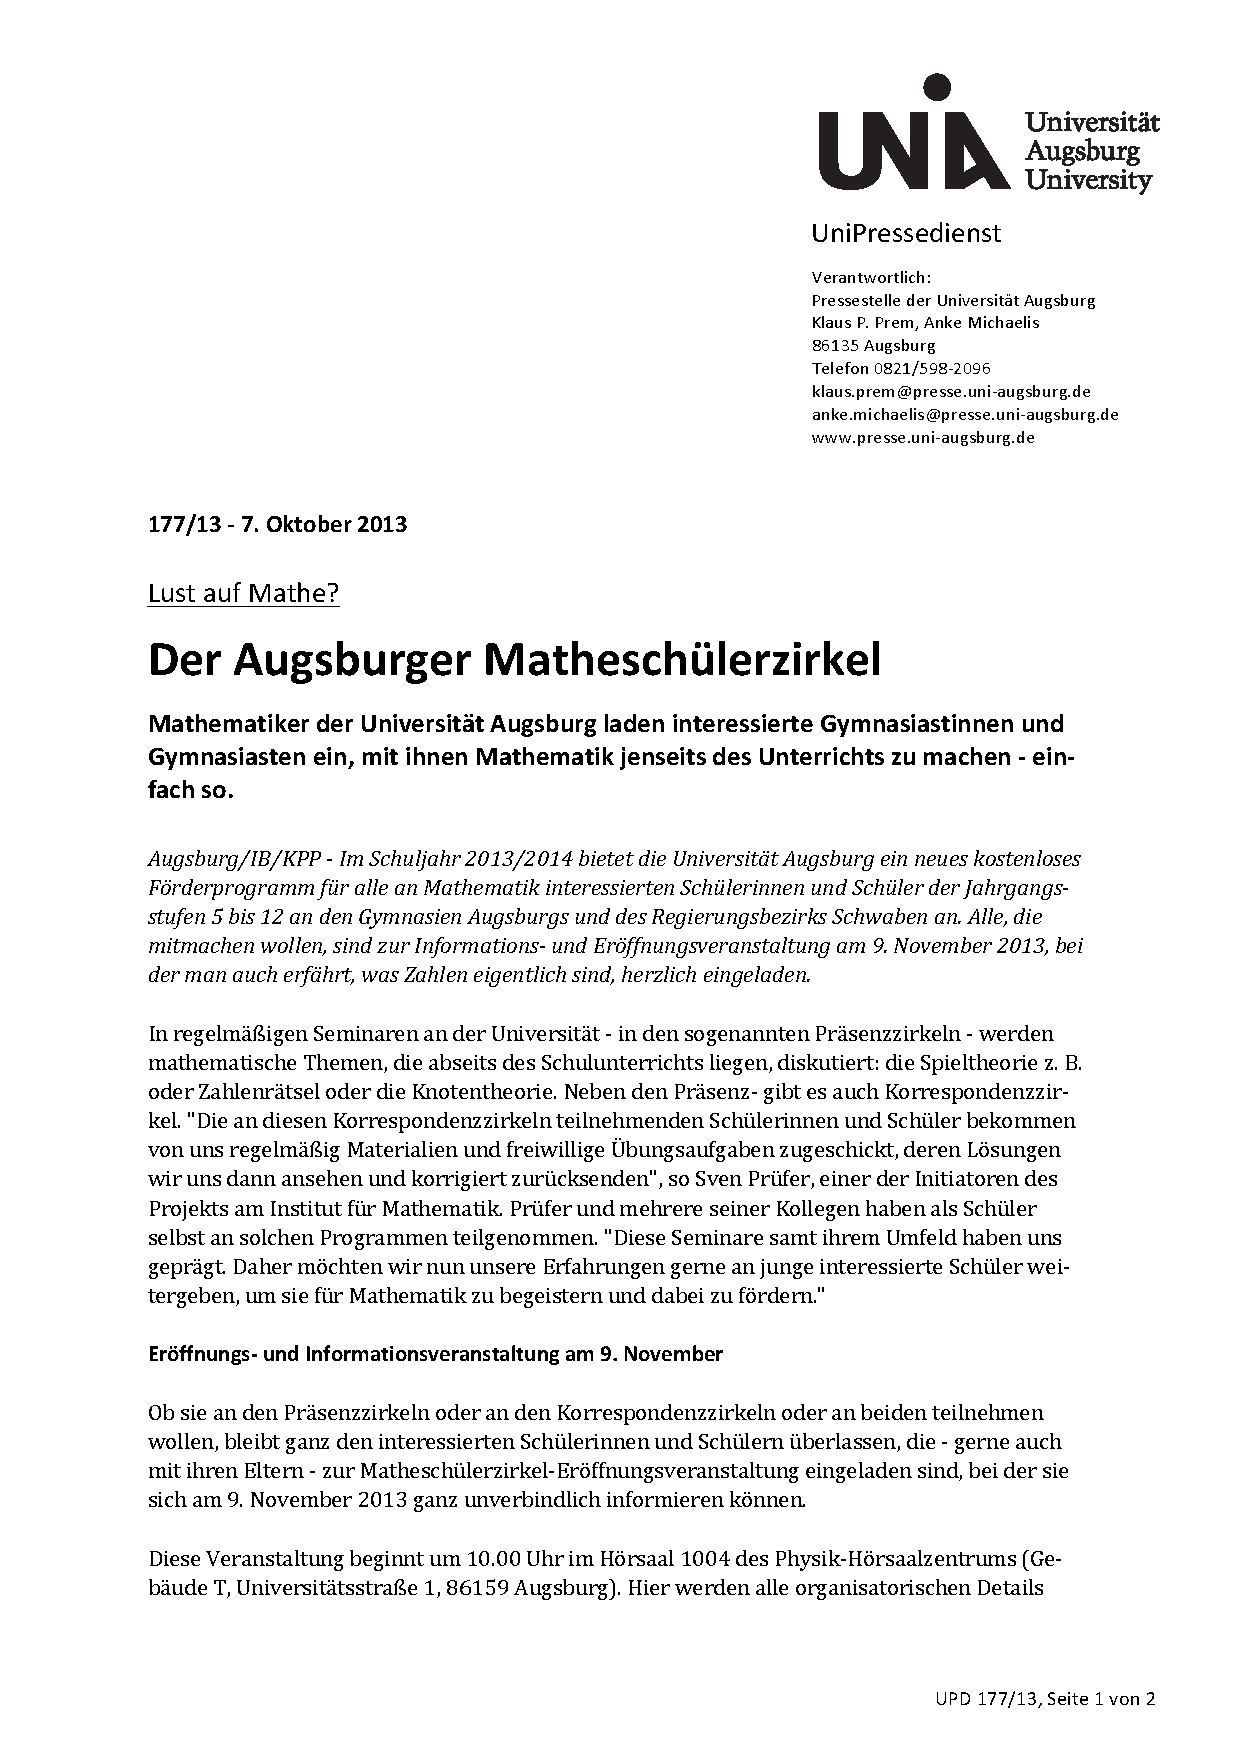
\includepdf[pages=1-2]{pressemitteilung-auftaktveranstaltung}

\hspace{-3.5cm}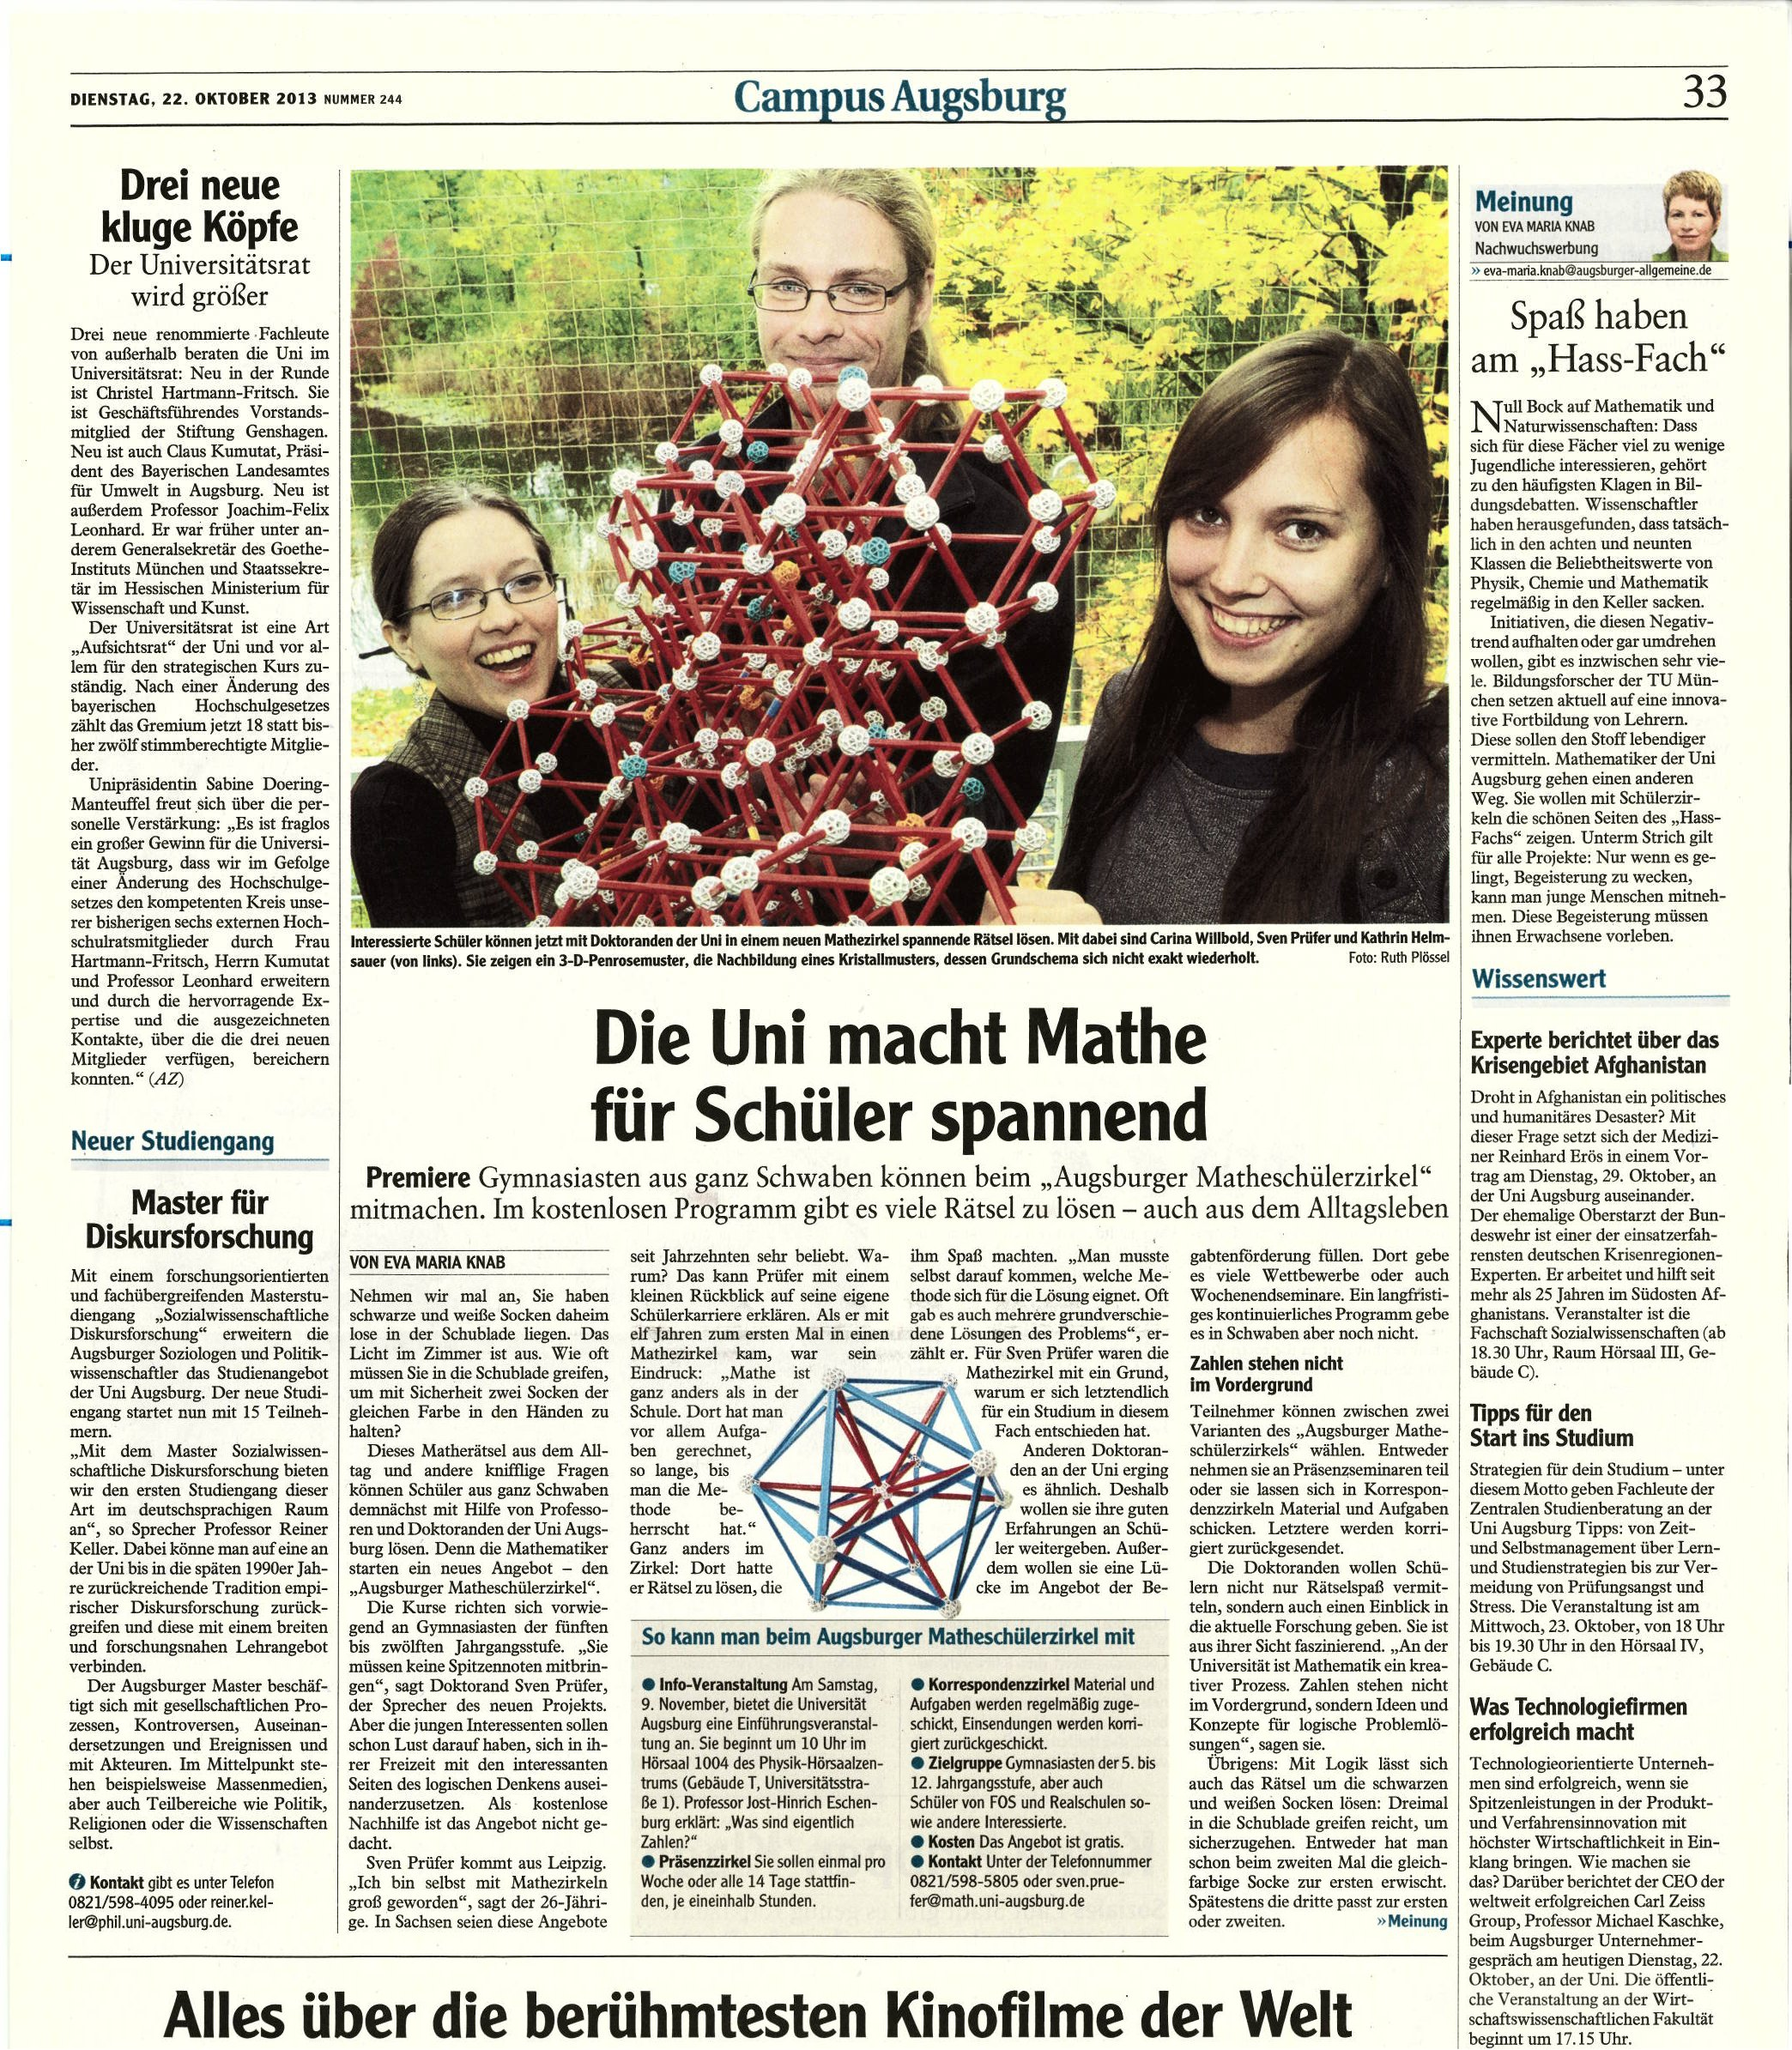
\includegraphics[scale=0.62]{Augsburger-Allgemeine-2013-10-22.jpeg}

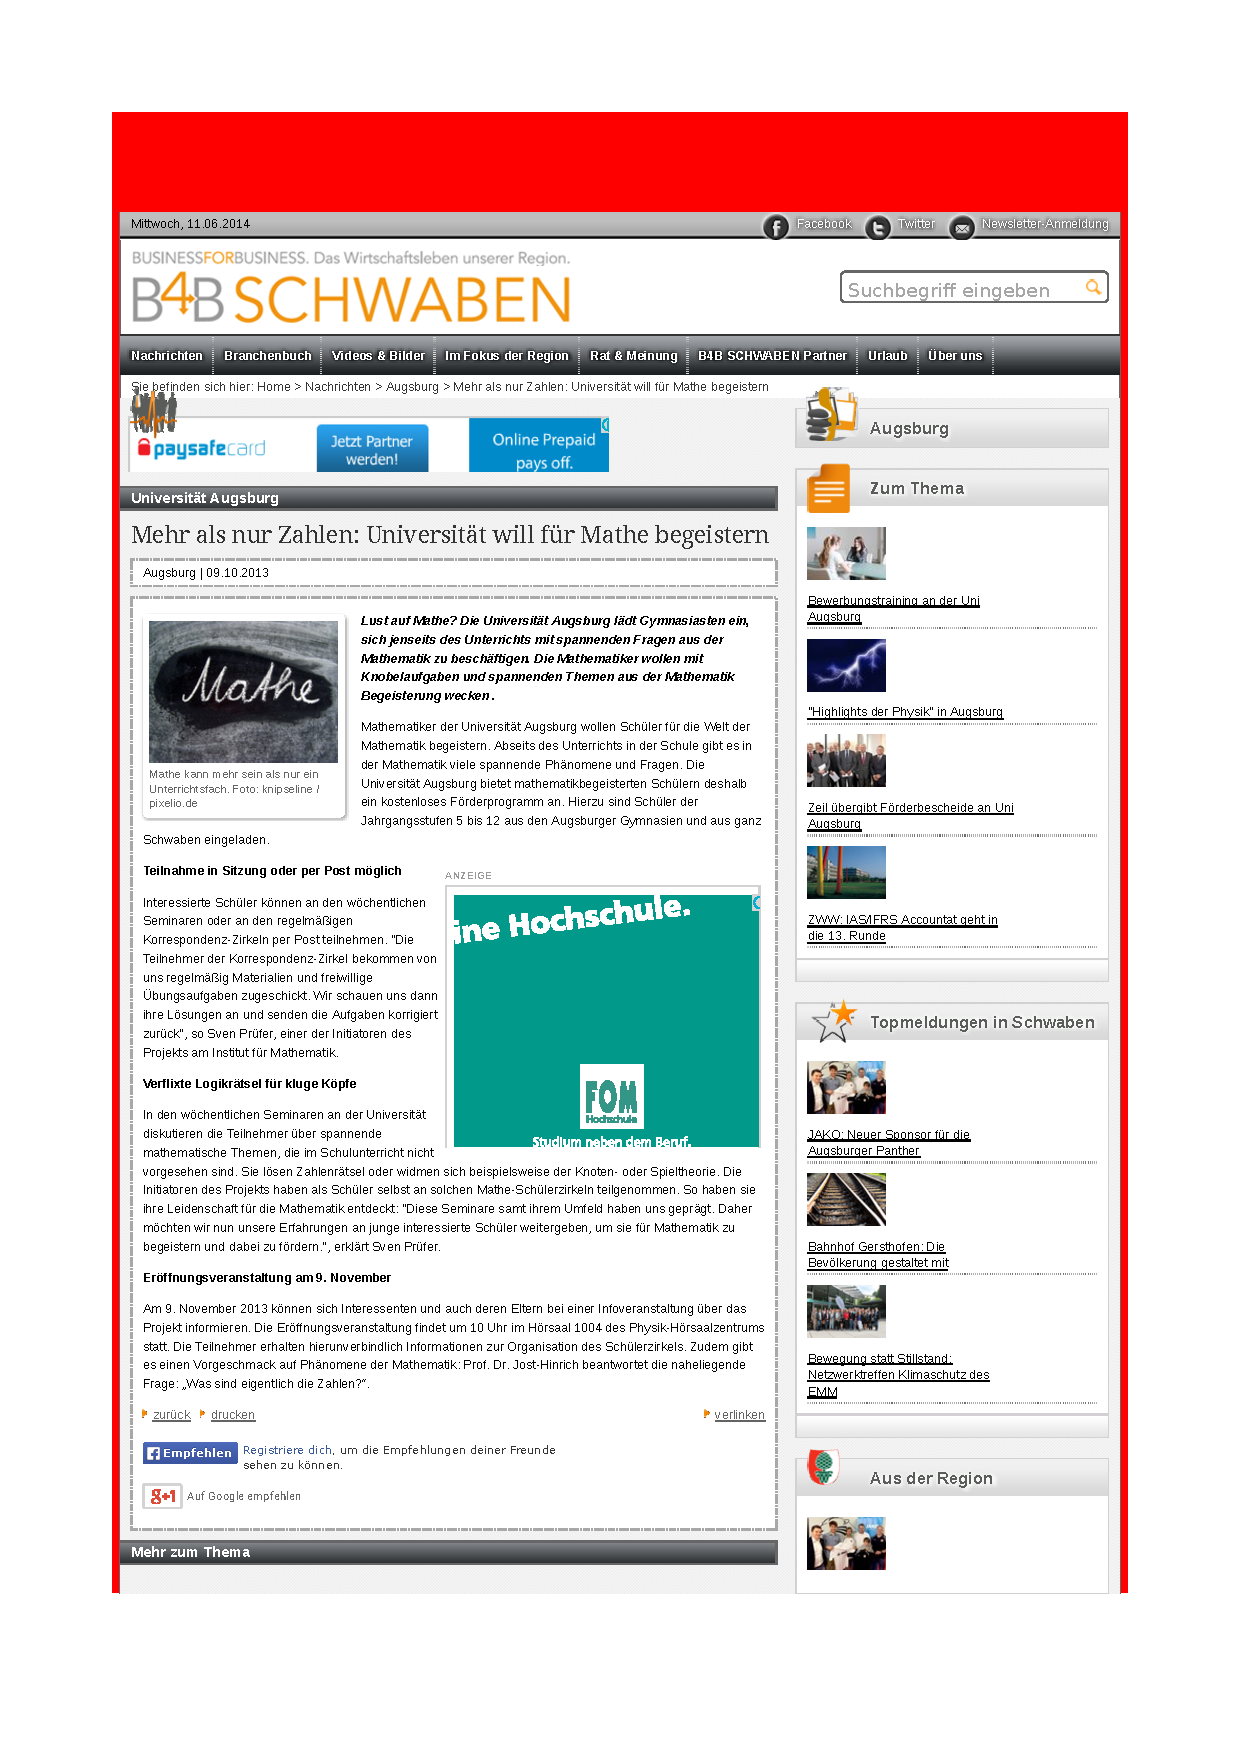
\includepdf{b4bschwaben-2013-10-09}

\end{document}
